
\documentclass[a4paper,10pt,english]{article}
\usepackage[utf8]{inputenc}
\usepackage[english]{babel}

\usepackage{amsmath,graphicx,varioref,verbatim,amsfonts,geometry}
\usepackage[thinc]{esdiff}
\usepackage[usenames,dvipsnames,svgnames,table]{xcolor}
\usepackage[colorlinks=false]{hyperref}

\usepackage{bm}

\setlength{\parindent}{0mm}
\setlength{\parskip}{1.5mm}

\usepackage{textcomp}
\definecolor{listinggray}{gray}{0.9}
\definecolor{lbcolor}{rgb}{0.9,0.9,0.9}

\usepackage{listings}

\lstdefinelanguage{python}
{
	morekeywords={print,abs,for,def,if,while,do,break,return,from,import,try,except,else,elif},
	sensitive=false,
	morecomment=[l]{\#}
}

\lstset{language=python,
	backgroundcolor=\color[rgb]{.95,.95,.95},
	numbers=left,xleftmargin=10pt,
	numberstyle=\tiny,stepnumber=1,numbersep=5pt,
	stringstyle=\color{red},
	basicstyle=\footnotesize \ttfamily,
	keywordstyle=\color{blue},
	commentstyle=\color{green},
	basewidth=0.60em,
	showstringspaces=false,
	captionpos=b,
	frame=single
}

\newcounter{subproject}
\renewcommand{\thesubproject}{\alph{subproject}}
\newenvironment{subproj}{
\begin{description}
\item[\refstepcounter{subproject}(\thesubproject)]
}{\end{description}}

%Lettering instead of numbering in different layers
% \renewcommand{\labelenumi}{\alph{enumi}}
\renewcommand{\thesubsection}{\alph{subsection}.}

\title{MEK1100 - Mandatory assignment 1}
\author{William Dugan}

\begin{document}

\maketitle

\section{Scaling}
A ball thrown with initial velocity $v_0$ and at an angle $\theta$ to the horizontal at time $t=0$ will follow the curve defined by
\begin{align}
    x(t) &= v_0 t \cos\theta \\
    y(t) &= v_0 t \sin\theta - \frac{1}{2} g t^2.
    \label{eq:1}
\end{align}

\subsection{}
The time taken for the ball to reach $y=0$ is
\begin{align*}
    y(t) &= 0 \\
    v_o t \sin\theta &= \frac{1}{2} g t^2 \\
    t &= \frac{2 v_0 \sin\theta}{g} = t_m
\end{align*}
The x-component at this time is
\begin{align*}
    x(t_m) &= \frac{2 v_0^2 \sin\theta\cos\theta}{g} \\
    &= \frac{v_0^2\sin(2\theta)}{g} = x_m
\end{align*}

\subsection{}
We introduce the following dimensionless variables:
\begin{align*}
    x^* &= \frac{x}{x_m} \implies x = x^* x_m \\
    y^* &= \frac{y}{x_m} \implies y = y^* x_m \\
\end{align*}
We insert these into (1) and get
\begin{align*}
    v_0 t \cos\theta &= x^* \frac{v_0^2 \sin(2\theta)}{g} \\
    x^* &= \frac{gt}{2 v_0 \sin\theta} \\
    v_0 t \sin\theta - \frac{1}{2} g t^2 &= y^* \frac{v_0^2 \sin(2\theta)}{g} \\
    y^* &= \frac{g(v_0 t \sin\theta - \frac{1}{2}gt^2)}{v_0^2 \sin\theta\cos\theta} \\
    y^* &= \frac{gt}{2v_0\cos\theta} - \frac{g^2t^2}{4v_0^2 \sin\theta\cos\theta} \\
    y^* &= \frac{gt}{2v_0\sin\theta} \cdot \frac{sin\theta}{\cos\theta} \cdot \left(1-\frac{gt}{2v_0\sin\theta}\right) \\
    y^* &= x^* \tan\theta (1-x^*)
\end{align*}
Scaling time is done by $t^* = t/t_m = x^*$. $\theta$ is dimensionless, hence we do not need to scale it. 

\subsection{}
\lstinputlisting{code/oppgave1.py}

\newpage
\begin{figure}[h!]
    \centering
    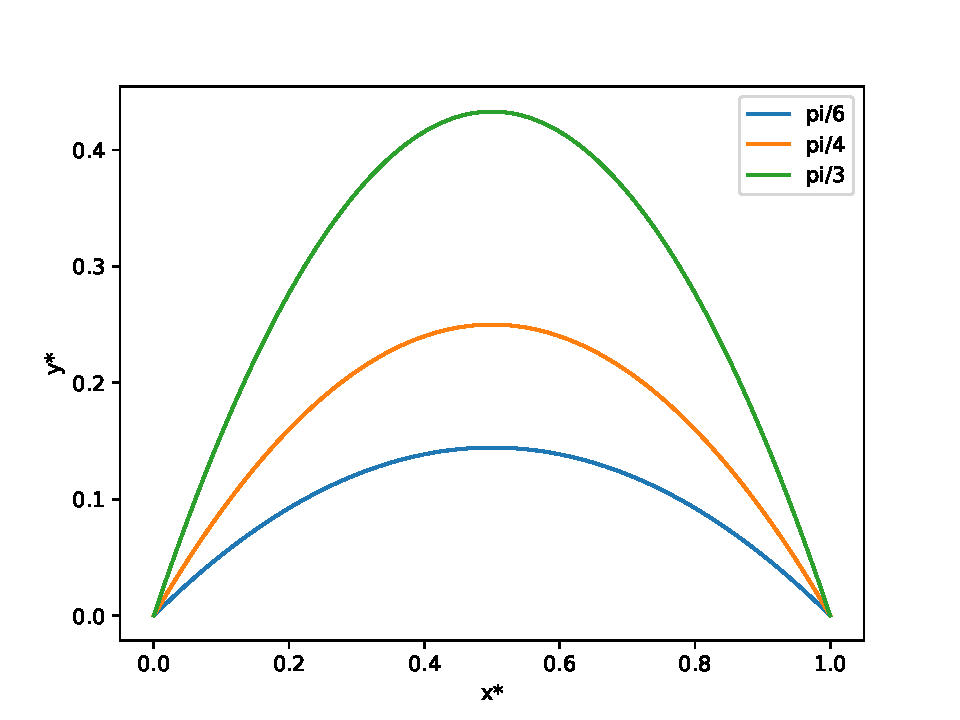
\includegraphics[scale=0.8]{figures/figure_1_c.pdf}
    \caption{Plot of $x^*$, $y^*$ for $\theta = \pi/6, \pi/4, \pi/3$.}
    \label{fig:figure_1_c}
\end{figure}
Since we have used dimensionless variables, the trajectory of the ball will only depend on the angle $\theta$. 

\section{Stream lines for a two-dimensional field}
We are given the velocity field
\begin{align}
    \bm{v} = v_x \bm{i} + v_y \bm{j} = xy \bm{i} + y \bm{j}.
    \label{eq:3}
\end{align}
\subsection{}
To find the stream lines we integrate both sides as described in chapter 2.4 in Gjevik \& Fagerland (2021).
\begin{align*}
    \int xy dy &= \int y dx \\
    \int dy &= \int\frac{1}{x} dx \\
    y &= \ln{|x|} + C
\end{align*}
It is clear that if $y=0$ the whole $x$-axis is a solution to the initial differential equation.

\newpage
\subsection{}
\begin{figure}[h]
    \centering
    \includegraphics[scale=0.4]{figures/figure_2_b_i.pdf}
    \caption{Hand-drawn stream lines for velocity field in \eqref{eq:3}}
    \label{fig:figure_2_b_i}
\end{figure}
The contour lines are defined when $y = \ln|x| + C$ is constant, meaning $z = \ln|x| - y$. All stagnation points will lie along the $x$-axis. 

\lstinputlisting{code/oppgave2.py}

See also \autoref{fig:figure_2_b_ii}  on next page.

\subsection{}
According to 4.6 in Gjevik \& Fagerland (2021), there is a stream function $\psi=\psi(x, y)$ if 
\begin{align}
    \nabla \cdot \bm{v} 
    = \frac{\partial v_x}{\partial x} + \frac{\partial v_y}{\partial y}
    = 0
\end{align}
We can calculate the divergence of $\bm{v}$ in \eqref{eq:3}.
\begin{align*}
    \frac{\partial v_x}{\partial x} + \frac{\partial v_y}{\partial y}
    = y + 1 \neq 0
\end{align*}
Hence, there is no $\psi$ for the given velocity field. 

\begin{figure}[h]
    \centering
    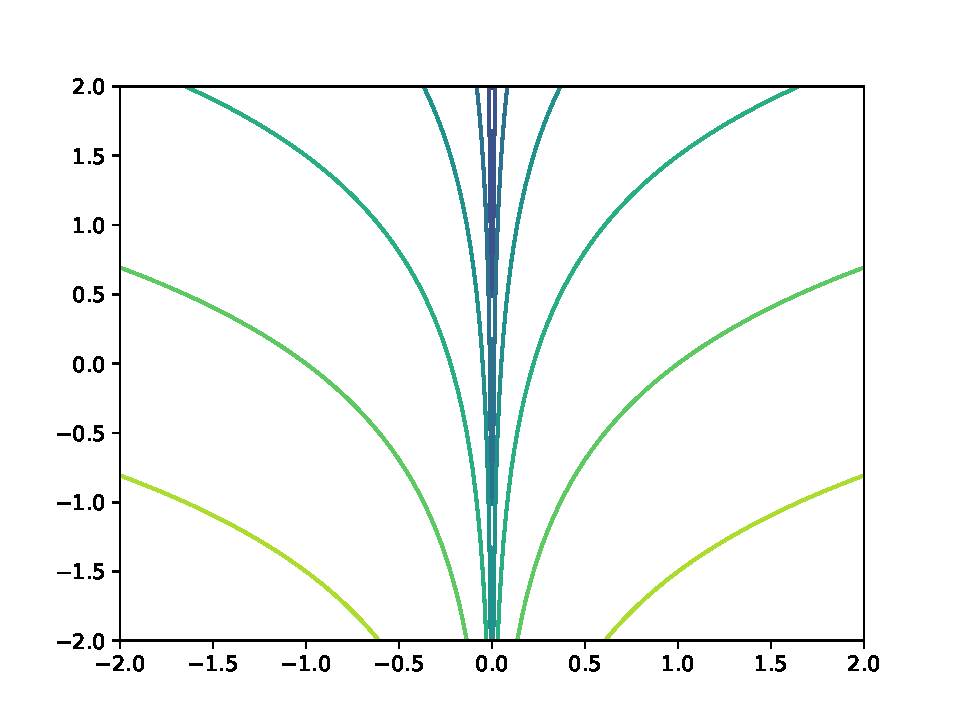
\includegraphics[scale=0.7]{figures/figure_2_b_ii.pdf}
    \caption{Stream lines drawn in python for velocity field in \eqref{eq:3}}
    \label{fig:figure_2_b_ii}
\end{figure}

\section{Another two dimensional stream field}
A velocity field in the $xy$-plane is given by $\bm{v} = v_x \bm{i} + v_y \bm{j}$ where 
\begin{align}
    v_x = \cos(x)\sin(y),\hspace{.3cm} v_y = -\sin(x)\cos(y).
    \label{eq:5}
\end{align}

\subsection{}
Divergence:
\begin{align*}
    \nabla \cdot \bm{v} = -\sin(s)\sin(y) + \sin(x)\sin(y) = 0
\end{align*}
Curl:
\begin{align*}
    \nabla \times \bm{v} 
    = \left( \frac{\partial v_x}{\partial x} - \frac{\partial v_y}{\partial y} \right)\bm{k}
    = (-2\cos(x)\cos(y))\bm{k}
\end{align*}

\newpage
\subsection{}
The given task was quite vague, so I simply plotted the field in python.
\lstinputlisting{code/oppgave3.py}
\vspace{-.5cm}
\begin{figure}[h]
    \centering
    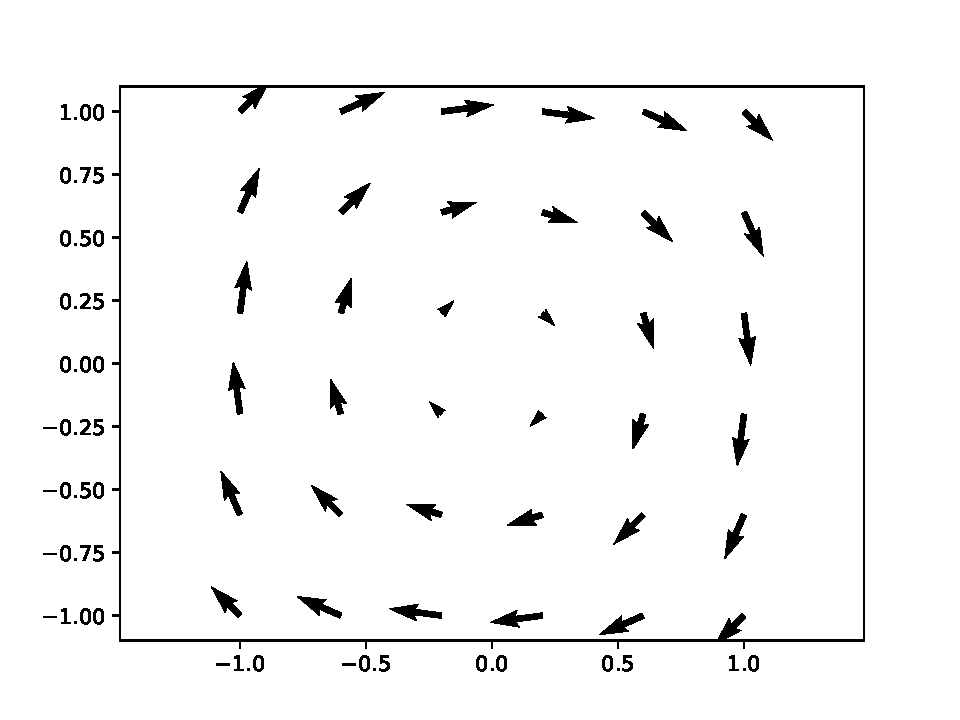
\includegraphics[scale=0.7]{figures/figure_3_b.pdf}
    \caption{Plot of $\bm{v}$ for $x, y \in[-1, 1]$}
    \label{fig:figure_3_b}
\end{figure}

\subsection{}
In this section, we will use the formula for a line integral of a vector field over a curve 
\begin{align}
    \int_C \bm{F} \cdot \bm{dr}
\end{align}

We separate the curve into four separate pieces. Consider the paramererisation $\bm{r}(t) = (t, -\pi/2)$ for $t\in[-\pi/2, \pi/2]$. Differentiating this we get $\bm{dr} = (1, 0)$. Hence, our integral is
\begin{align*}
    & \int_{-\pi/2}^{\pi/2} (v_x, v_y) \cdot (1, 0) dt \\
    = &\int_{-\pi/2}^{\pi/2} \cos(t)\sin(-\pi/2) dt \\
    = &\left[ -sin(t)\right]_{-\pi/2}^{\pi/2} \\
    = &-2
\end{align*}
We perform similar calculations for the three other sides. This results in the circulation around the square defined as $-\pi/2 \leq x, y \leq \pi/2$ to be $-2*4 = -8$.

\subsection{}
To check if 
\begin{align}
    \psi = \cos(x)\cos(y)
    \label{eq:psi}
\end{align}
is a valid stream function for $\bm{v}$, we turn to 4.6 in Gjevik \& Fagerland (2021) once again. We have that 
\begin{align}
    v_x = -\frac{\partial \psi}{\partial y}, 
    \hspace{.3cm} v_y = \frac{\partial \psi}{\partial x}
\end{align}
if $\psi(x, y)$ is a stream function for $\bm{v} = (v_x, v_y)$. We test for our given $\psi$ and $\bm{v}$:
\begin{align*}
    \frac{\partial \psi}{\partial y} &= -\cos(x)\sin(y) = - v_x \\
    \frac{\partial \psi}{\partial x} &= \sin(x)\cos(y) = v_y
\end{align*}
which shows that \eqref{eq:psi} is a stream function for \eqref{eq:5}.

\subsection{} \label{3e}
To find the Taylor approximation of $\psi(0, 0)$ we use the formula stated in chapter 2.2 in Gjevik \& Fagerland (2021).
\begin{align*}
    f(x, y) \cong f(x_0, y_0) 
    &+ \frac{\partial f}{\partial x}(x_0, y_0)(x-x_0)
    + \frac{\partial f}{\partial y}(x_0, y_0)(y-y_0) \\
    &+ \frac{1}{2}\frac{\partial^2 f}{\partial x^2}(x_0, y_0) (x-x_0)^2
    + \frac{1}{2}\frac{\partial^2 f}{\partial y^2}(x_0, y_0) (y-y_0)^2 \\
    &+ \frac{\partial^2 f}{\partial x \partial y} (x-x_0)(y-y_0)
\end{align*}
To save on some typing, I will only include the parts that do not become zero. We use $(x_0, y_0) = (0, 0)$.
\begin{align*}
    \psi(0, 0) &= 1 \\
    \frac{\partial^2 \psi}{\partial x^2} = -\cos(x)\cos(y) 
        \implies \frac{\partial^2 \psi}{\partial x^2} (0, 0) &= -1 \\
    \frac{\partial^2 \psi}{\partial y^2} = -\cos(x)\cos(y) 
        \implies \frac{\partial^2 \psi}{\partial y^2} (0, 0) &= -1 \\
\end{align*}
If we insert these values into our formula we get
\begin{align}
    \psi (x, y) \cong 1 - \frac{x^2}{2} - \frac{y^2}{2}
    \label{eq:9}
\end{align}

\section{Stream lines and velocity field in Python}
\subsection{}
\verb|strlin.py|:
\lstinputlisting{code/strlin.py}

\begin{figure}[h]
    \centering
    \begin{minipage}{0.5\textwidth}
        \centering 
        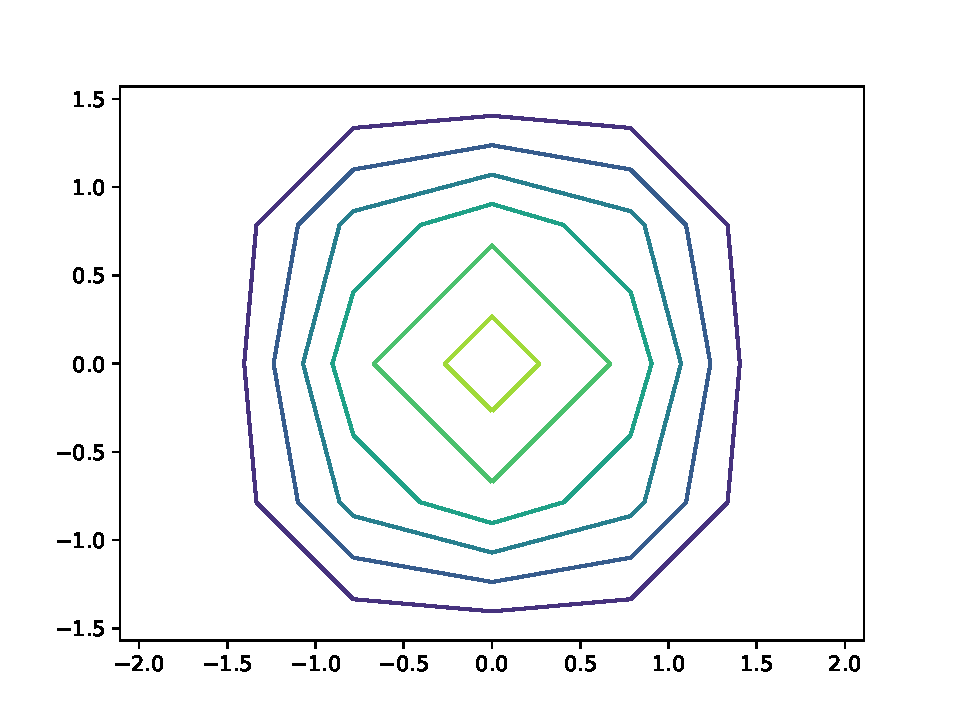
\includegraphics[scale=.5]{figures/figure_4_a_i.pdf}
    \end{minipage}\hfill
    \begin{minipage}{0.5\textwidth}
        \centering 
        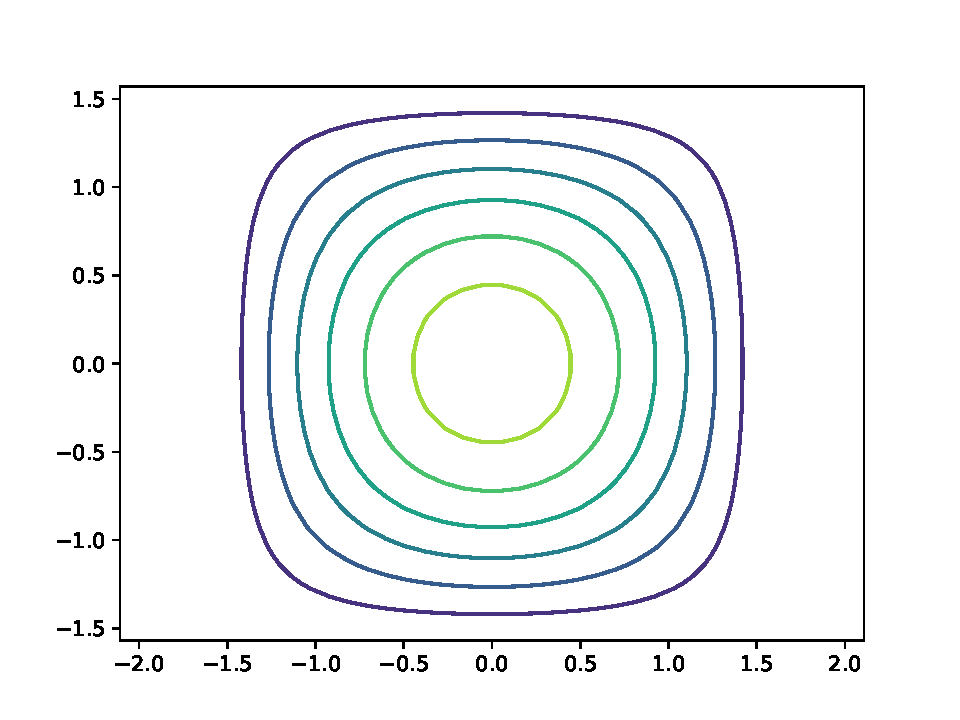
\includegraphics[scale=.5]{figures/figure_4_a_ii.pdf}
    \end{minipage}
    \caption{Showing streamlines for $n=5, 30$.}
    \label{fig:stremalines}
\end{figure}
We observe that if we use a higher $n$, such as 30, the shape is more close to the circles described by \eqref{eq:9}. 

\subsection{}
\verb|velfield.py|:
\lstinputlisting{code/velfield.py}
\verb|vec.py|:
\lstinputlisting{code/vec.py}

\begin{figure}[h]
    \centering
    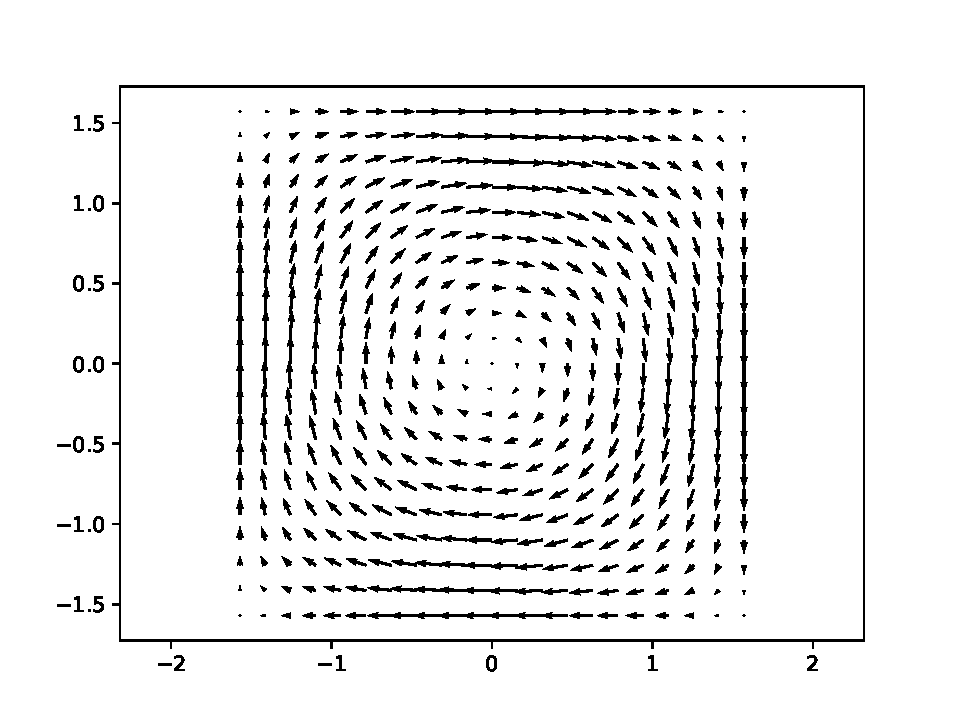
\includegraphics[scale=.7]{figures/figure_4_b.pdf}
    \caption{Plot of velocity field with $n=21$.}
    \label{fig:figure_4_b}
\end{figure}

\end{document}
